% LaTeX template for Lab Reports
% Copyright (C) 2014 Julian Coy

%% CHANGE REPORT TITLE HERE
\newcommand{\reporttitle}{
 Rate Monotonic Analysis
}

%% HEADER/PREAMBLE INFORMATION

% "The font should be 11pt Times New Roman"
\documentclass[11pt]{report}
\usepackage[T1]{fontenc}
\usepackage[utf8]{inputenc}

\usepackage{mathptmx}               

% "The body of the paper should use 1" margins on all sides."
\usepackage[margin=1in]{geometry}

% "Pages must be numbered, starting with 1 on the first page in the body of the report.
% The cover page should not be numbered. 
% Page numbers should be in the bottom-right corner of the page."
\usepackage{fancyhdr}
\pagestyle{fancy}
\fancyhead{}
\fancyfoot{}
\renewcommand{\headrulewidth}{0pt}
\fancyfoot[R]{\thepage}

% Set up customized spacing
\usepackage{setspace}

% Allows for Trademark Symbols
\usepackage{textcomp}

% Remove spacing between items in lists
\usepackage{enumitem}

% Remove extra spacing between titles of sections and subsections
\usepackage{titlesec}
\titlespacing\section{0pt}{10pt}{10pt}
\titlespacing\subsection{0pt}{10pt}{10pt}
\titlespacing\subsubsection{0pt}{0pt plus 4pt minus 2pt}{0pt plus 2pt minus 2pt}

% Setup the specialized chapter section for the Abstract
\titlespacing\chapter{0pt}{0pt plus 4pt minus 2pt}{0pt plus 2pt minus 2pt}
\titleformat{\chapter}[block]{\centering\Huge}{}{}{}{}


% Set up math
\usepackage{amsmath}
\usepackage{amsfonts}
\usepackage{amssymb}

% Set up graphics
\usepackage{graphicx}
\usepackage{float}

% Set up tables
\usepackage{tabularx}
\usepackage{booktabs}

% Set up code blocks
% or not...

\usepackage{listings}
\usepackage{color}

\definecolor{dkgreen}{rgb}{0,0.6,0}
\definecolor{gray}{rgb}{0.5,0.5,0.5}
\definecolor{mauve}{rgb}{0.58,0,0.82}

\lstset{frame=tb,
  language=C,
  aboveskip=3mm,
  belowskip=3mm,
  showstringspaces=false,
  columns=flexible,
  basicstyle={\small\ttfamily},
  numbers=none,
  numberstyle=\tiny\color{gray},
  % keywordstyle=\color{blue},
  commentstyle=\color{dkgreen},
  stringstyle=\color{mauve},
  breaklines=true,
  breakatwhitespace=true
  tabsize=3
}

%% START OF DOCUMENT

\begin{document}

% "The main body of text should use 1.5 spacing"
\begin{spacing}{1.5}

% Suppress page numbering on first page
\thispagestyle{empty}

\begin{scshape}

% Title
% "The title should be centered and written in approximately 22pt font."
\vspace*{30pt}
{
\Huge
\begin{center}
    \reporttitle
\end{center}
}
\vspace{30pt}

% Team Number
% "The Team number should be centered and written several lines below the title and should use a
% similar size font as the title."
{
\Large
\begin{center}
  Lab 6 Report for ECE468 \\
  Embedded Computing
\end{center}
}
\vspace{30pt}
% Team Members
% "Directly below the team identifier, team members should be listed alphabetically by last name, one
% per line, in approximately 14pt font. The column of names should be approximately centered on
% the page, but the names within the column should be left justified (so they all start at the same
% horizontal position)."
{
\Large 
\begin{center}
  Submitted by \\
  Julian Coy
\end{center}
}
\vspace{120pt}

{
\Large
\begin{center}
  Undergraduate of Electrical \& Computer Engineering \\
  Clemson University
\end{center}
}
\vspace{30pt}

{
\Large
\begin{center}
  \today
\end{center}
}

\end{scshape}

% New page and reset page numbering
\clearpage

%% START EDITS BELOW %%

\vspace{15pt}
  \setcounter{chapter}{1}
  \chapter*{Abstract}
  \label{cha:abstract}
\vspace{72pt}

An Inertial Navigation System (INS) is a real-time shipboard avionic system. It has strict time constraints for providing information to other shipboard devices. For example, an INS tracks attitude, geographic position, velocity, distance and displacement.  The goal of this experiment is to use Rate Monotonic Analysis do determine if the system is schedulable on a Motorola MC68302 microcontroller that is implementing a priority ceiling protocol.

\thispagestyle{empty} % clear page number
\clearpage
\setcounter{page}{1}

\section*{\scshape Introduction} %(0.5 pages)
\label{cha:introduction}

There are specific timing constraints that are in place for each subtask in the system.  Figure \ref{fig:timing} shows the time constraints of specific features.  The period is the interval between task completions.  In essence, this number lets us know when a specific task needs to complete execution.

\vspace{15px}
\begin{figure}[H]
    \centering
    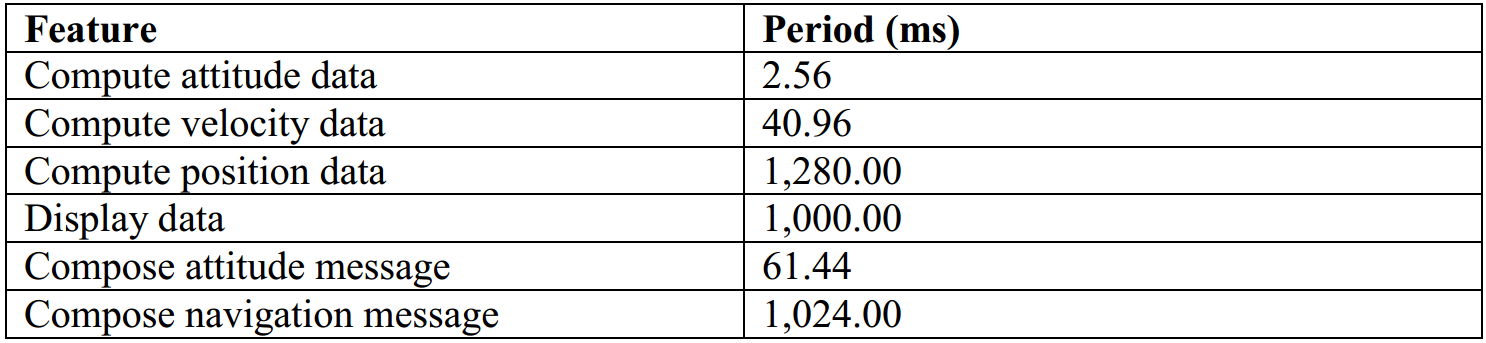
\includegraphics[width=0.85\textwidth,keepaspectratio]{timing}
    \caption{Timing Constraints}
    \label{fig:timing}
\end{figure}

When switching tasks, the system will incur and overhead delay of 153$\mu$s.  Below in Figure \ref{fig:resources}, you can see the specific resource usage required by each task.

\vspace{15px}
\begin{figure}[H]
    \centering
    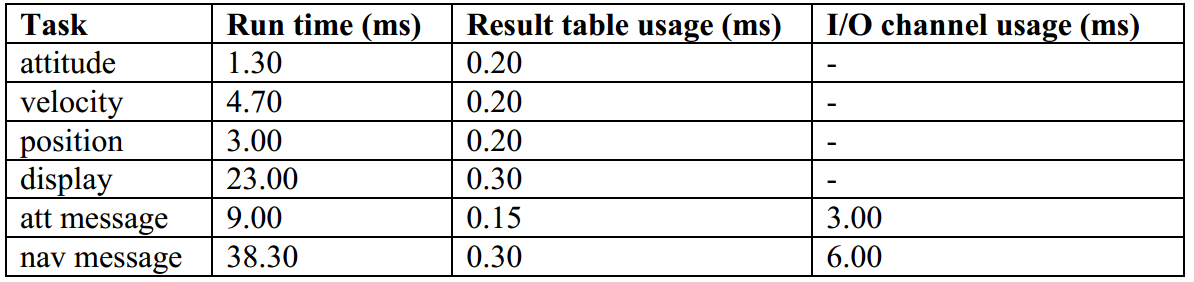
\includegraphics[width=0.85\textwidth,keepaspectratio]{resources}
    \caption{Resource Usage}
    \label{fig:resources}
\end{figure}

Each task will share the same result table, and two will share an I/O channel.  These resources will need to be modeled as semaphorically protected for a proper RMA analysis.  Due to the semaphores that will be present, it becomes necessary to analyze each task with regard to its maximum blocking time.  This time is calculated from the large of two statistics: direct blocking and pass-through blocking.  Direct blocking occurs when a lower priority task holds a needed resource.  Pass-through blocking occurs when a medium priority task is blocked by a lower priority task that has inherited a higher priority, due to a share resource constraint.

\section*{\scshape Experiment} %(0.5 pages)
\label{cha:experiment}

To test the schedulability of this system, a C program was written to perform RMA analysis upon the data sets provided.  The C program followed the rate monotonic analysis formulas provided by Dr. Hoover in class.

\section*{\scshape Results} %(0.5 pages)
\label{cha:results}

The system is schedulable with k = 1 and l = 117.  The following output is the verbose results of the program when supplied with the data provided earlier.  The blocking values, and other information were hard coded into the program. See Code section for the program source.

\section*{Output}
\begin{lstlisting}
Testing for possible scheduling...

Pass for i: 1
  Fail with i: 2  k: 1  l: 1
  Fail with i: 2  k: 1  l: 2
  Fail with i: 2  k: 1  l: 3
Pass for i: 2
  Fail with i: 3  k: 1  l: 1
  Fail with i: 3  k: 1  l: 2
  ...
  Fail with i: 3  k: 1  l: 14
  Fail with i: 3  k: 1  l: 15
Pass for i: 3
  Fail with i: 4  k: 1  l: 1
  Fail with i: 4  k: 1  l: 2
  ...
  Fail with i: 4  k: 1  l: 58
  Fail with i: 4  k: 1  l: 59
Pass for i: 4
  Fail with i: 5  k: 1  l: 1
  Fail with i: 5  k: 1  l: 2
  ...
  Fail with i: 5  k: 1  l: 114
  Fail with i: 5  k: 1  l: 115
Pass for i: 5
  Fail with i: 6  k: 1  l: 1
  Fail with i: 6  k: 1  l: 2
  ...
  Fail with i: 6  k: 1  l: 115
  Fail with i: 6  k: 1  l: 116
Pass for i: 6

System is schedulable with k: 1 and l: 117.
\end{lstlisting}

\lstset{
    keywordstyle=\color{blue},
}

\section*{Lab 6: Code}
\begin{lstlisting}
#include <stdio.h>
#include <stdlib.h>
#include <errno.h>
#include <string.h>
#include <stdbool.h>
#include <math.h>

#define OVERHEAD 0.153

typedef struct _task {
  double  runtime, period;
  double  semaphore[2];
  double  max_blocking;
} TASK;

void
printErr ( char *, int );

void
RMA ( TASK [], int, bool );

int
main ( int argc, char *argv[] )
{
  //////////////////////////
  /// SET DEFAULT VALUES ///
  //////////////////////////

  bool VERBOSE = false;

  //////////////////////////
  /// VERIFY/PARSE INPUT ///
  //////////////////////////

  int i;

  for (i = 1; i < argc; i++)
  {
    if (strcmp(argv[i], "-v") == 0)
      VERBOSE = true;
    else
      printErr(argv[i], EINVAL);
  }

  /* /////////////|\\\\\\\\\\\\\ */
  /* |||      DO STUFFS      ||| */
  /* \\\\\\\\\\\\\|///////////// */


  // Build a task set
  TASK task[6];

  task[0].runtime      = 1.3;
  task[0].period       = 2.56;
  task[0].semaphore[0] = 0.2;
  task[0].semaphore[0] = 0.0;
  task[0].max_blocking = 0.3;

  task[1].runtime      = 4.7;
  task[1].period       = 40.96;
  task[1].semaphore[0] = 0.2;
  task[1].semaphore[0] = 0.0;
  task[1].max_blocking = 0.3;

  task[2].runtime      = 9.0;
  task[2].period       = 61.44;
  task[2].semaphore[0] = 0.15;
  task[2].semaphore[0] = 3.00;
  task[2].max_blocking = 6.00;

  task[3].runtime      = 23.0;
  task[3].period       = 1000.0;
  task[3].semaphore[0] = 0.30;
  task[3].semaphore[0] = 0.0;
  task[3].max_blocking = 6.00;

  task[4].runtime      = 38.3;
  task[4].period       = 1024.0;
  task[4].semaphore[0] = 0.30;
  task[4].semaphore[0] = 6.00;
  task[4].max_blocking = 0.2;

  task[5].runtime      = 3.0;
  task[5].period       = 1280.0;
  task[5].semaphore[0] = 0.2;
  task[5].semaphore[0] = 0.0;
  task[5].max_blocking = 0.0;

  RMA( task, 6, VERBOSE );

  exit(0);
}

//function definitions

void
RMA( TASK task[], int count, bool VERBOSE )
{
  int i, j, k, l;
  int storedk, storedl;

  double LHS, RHS, inner;

  bool SCHEDULABLE;

  if ( VERBOSE ) printf( "Testing for possible scheduling...\n\n" );

  for ( i = 1; i <= count; i++ )
  // i iterates from 1 to n
  {
    SCHEDULABLE = false;
    for ( k = 1; k <= i; k++ )
    // k iterates from 1 to i
    {
      for ( l = 1; l <= (int) floor( task[i-1].period / task[k-1].period ); l++ )
      // k iterates from 1 to floor of Ti / Tk
      {
        // setup RHS and LHS for maths
        LHS = 0.0; // clear for loops
        RHS = (l) * task[k-1].period; // l * Tk

        // if ( VERBOSE ) printf( "\t\tLHS = " );

        // peform summation loop
        for ( j = 1; j < i; j++ )
        // sum from j=1 to i-1
        {
          inner = ( task[j-1].runtime + OVERHEAD );
          inner *= (int) ceil( l * task[k-1].period / task[j-1].period );
          LHS += inner;
        }

        // add in runtimes and blocking
        LHS = LHS + ( task[i-1].runtime + OVERHEAD + task[i-1].max_blocking );

        if ( LHS <= RHS ) {
          // set conditions to break two inner loops and continue i
          storedl = l;
          storedk = k;
          l = (int) floor( task[i-1].period / task[k-1].period ) + 1;
          k = i + 1;
          if ( VERBOSE ) printf( "Pass for i: %d\n", i );
          SCHEDULABLE = true;
        } else {
          if ( VERBOSE ) printf( "\tFail with i: %d\tk: %d\tl: %d\n", i, k, l );
        }

      } // end l
    } // end k
    if ( !SCHEDULABLE )
    {
      if ( VERBOSE ) printf( "\n" );
      printf ( "System is unschedulable at i: %d.\n", i );
      if ( VERBOSE ) printf( "\n" );
      exit(1);
    }
  } // end i

  if ( SCHEDULABLE )
  {
    if ( VERBOSE ) printf( "\n" );
    printf( "System is schedulable with k: %d and l: %d.\n", storedk, storedl );
    if ( VERBOSE ) printf( "\n" );
  }
}

void
printErr(char *str, int err)
{
  errno      = err;
  char *msg  = (char *)"Error:\n    ";
  char *pstr = NULL;
  pstr       = (char *)malloc(strlen(str) + strlen(msg));

  strcat(pstr, msg);
  strcat(pstr, str);
  perror(pstr);

  exit(err);
}
\end{lstlisting}

%% END EDITS HERE %%

\end{spacing}

\end{document}

%%%%%%%%%%%% Extra stuff for use later

% \begin{itemize}[noitemsep,nolistsep]
%     \item \emph{Choose off-the-shelf parts} rather than self-made parts whenever possible.
%     \item \emph{Reuse and expand on open-source software libraries} to avoid spending time writing code that duplicates functionality that already exists elsewhere (and is likely more robust).
%     \item \emph{Keep the hardware simple} by using the least amount of hardware necessary for operation to avoid additional potential points of failure.
%     \item \emph{Modularize systems and components}. Each component should do one thing and do it well.
% \end{itemize}
% Figure \ref{BlockDiagram} shows a block diagram of the subsystems used in our design.

% \begin{figure}[H]
%     \centering
%     \caption{Block Diagram of Subsystems}
%     \label{BlockDiagram}
% \end{figure}
%     {
%     \centering
%       \includegraphics[width=\textwidth]{CostAccounting}
%     }